%Edit 0022 ZZZ to report number nnnn 
%Edit 3.3.2 YYMILE to milestone number m.m.m
%Edit Report on design patterns specifications and prototypes YYTITLE to report title - Words Start with Caps
\documentclass[11pt,twoside,a4paper]{article}
%%======================================================================
%% PACKAGES:
%%
%\usepackage{times}               % Times+Helvetica+Courier fonts
\usepackage{helvet}              % helvetica + cmr
\usepackage{fancyhdr}       % package for headers/footers
\usepackage{amsmath}
\usepackage{amssymb}
\usepackage{graphicx}            % Graphics.
%\usepackage{a4}                  % page layout to fit A4
%\usepackage{lastpage}            % get page no of last page
%\usepackage{ifthen}              % logical branching
\usepackage{hyperref}            %insert hyper-links
\usepackage{latexsym}
% uncomment the following to override auto page total
%\pptotal{20}
%%======================================================================

% ensure sans-serif font used throughout
\renewcommand{\familydefault}{\sfdefault}

\newcommand{\culhamissueno}{1.00}%<==edit
\newcommand{\culhamshorttitle}{CD/EXCALIBUR-FMS/0023}%<==edit
\newcommand{\Sec}[1]{Section~\ref{sec:#1}}
\newcommand{\Fig}[1]{Figure~\ref{fig:#1}}
\newcommand{\Tab}[1]{Table~\ref{tab:#1}}
\newcommand{\Eq}[1]{Equation~(\ref{eq:#1})}
\newcommand{\Eqs}[2]{Equations(\ref{eq:#1}) and~(\ref{eq:#2})}
\newcommand{\Figs}[2]{Figures~\ref{fig:#1}--~\ref{fig:#2}}
%Bold lc for script names, tt for computer code and file-names
%\F{NEPTUNE} always in caps
\newcommand{\F}[1]{\textsc{#1}}
\newcommand{\B}[1]{\textbf{#1}}
\newcommand{\T}[1]{{\tt #1}}
\newcommand{\V}[1]{\mathbf{#1}}
\newcommand{\I}[1]{\textit{#1}}
\newcommand{\nep}{\textsc{NEPTUNE}}
\newcommand{\exc}{\textsc{E}x\textsc{CALIBUR}}
\newcommand{\Papp}{Proxyapp}
\newcommand{\papp}{proxyapp}



%%======================================================================

%% REPORT COVER PAGE Information

\newcommand{\culhamtitle}{\LARGE Report on design patterns specifications and prototypes  \\[1.0\baselineskip] M3.3.2 }%<==edit

%%QA BOX information -- change following as needed
\newcommand{\culhamboardname}{Martin O'Brien}%<==edit
\newcommand{\culhamcontactname}{Rob Akers}%<==edit
\newcommand{\culhamauthor}{Wayne Arter}%<==edit
\newcommand{\culhamauthora}{Ed Threlfall}%<==edit
\newcommand{\culhamauthorb}{Joseph Parker}%<==edit
\newcommand{\culhamauthorc}{Stan Pamela}%<==edit
%\newcommand{\culhamcontacttel}{Telephone: 01235 466498}
%\newcommand{\culhamcontactemail}{Email: rob.akers@ukaea.uk}

\newcommand{\culhamdate}{12 August 2020}%<=edit
\newcommand{\culhamdatea}{16 August 2020}%<=edit
\newcommand{\culhamdateb}{12 August 2020}%<=edit

% reproduce Rob's page size

\setlength{\textheight}{220.0mm}
\setlength{\textwidth}{165.0mm}
\setlength{\topmargin}{0.0mm}
\setlength{\oddsidemargin}{0.0mm}
\setlength{\evensidemargin}{\oddsidemargin}
\setlength{\parindent}{0mm}
\addtolength{\parskip}{0.5\baselineskip}
\setlength{\topsep}{0pt}
\setlength{\itemsep}{0pt}

%%======================================================================
\begin{document}

%Titlepage comes out wrong size, but should look right apart from
% picture which cannot be wider than c.150mm.
% To produce conforming report rp1pub.pdf
% remove title page by commenting out lines ending in %<==omit, then
% sed -e '/<==omit$/s/^/%/' < rp1.tex > rp1omit.tex
% pdflatex rp1omit;bibtex rp1omit; pdflatex rp1omit
% pdfunite cover.pdf rp1omit.pdf rp1pub.pdf 
\begin{titlepage}%<==omit
\vspace*{-30mm}%<==omit

\includegraphics[width=2.5cm]{../corpics/cofaplus} \\[2.0\baselineskip]%<==omit
{\LARGE {\textbf{\textsf{ExCALIBUR}}}}\\[2.0\baselineskip]%<==omit
{\LARGE \culhamtitle } \\[2.0\baselineskip]%<==omit
{\textbf{\textsf{Abstract}}}\\%<==omit
The report describes work for \exc \ project \nep \ %<==omit
at Milestone 3.3.2. %<==omit
The report describes equations for \exc \ project \nep \ \Papp s.  
The numbering of the systems follows that of the \nep\ Science Plan, so 
that those listed under FM-WP2 are denoted 2-1, 2-2, etc., and 
under FM-WP3 as 3-1, 3-2, etc. It is a living document to which further equation 
systems will be added throughout the course of the project.
%<==omit
%<==omit
\vfill%<==omit
\centerline{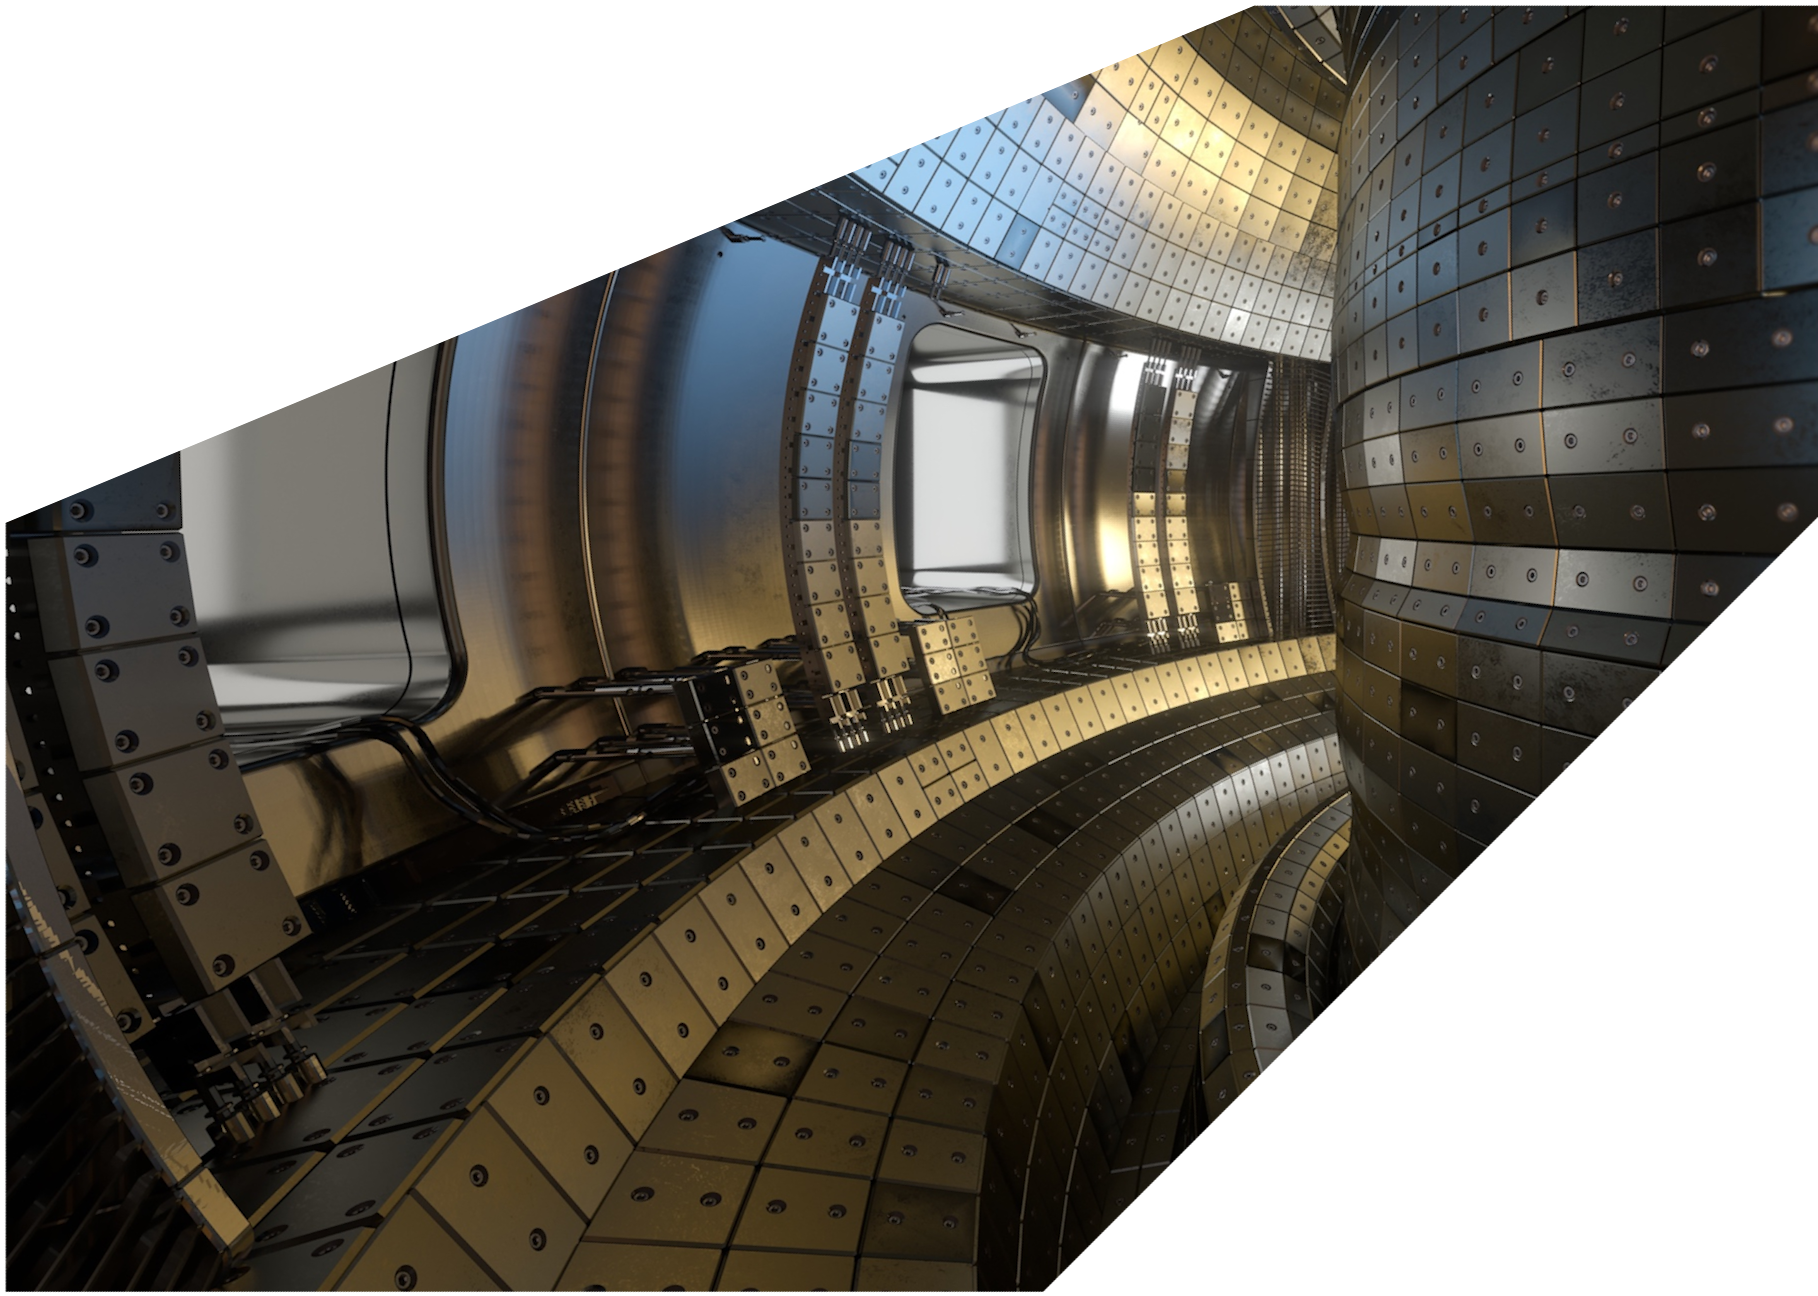
\includegraphics[width=0.9\textwidth]{../corpics/tokintcrop}}%<==omit
\end{titlepage}%<==omit

\hspace{-30mm}\begin{table}[h]
\sffamily
\begin{center}
\textbf{\textsf{UKAEA REFERENCE AND APPROVAL SHEET}}
\begin{tabular}{||p{5.7cm}|p{4.7cm}|p{5.0cm}||}
\hline
\hline
& Client Reference: &  \\
\hline
& UKAEA Reference: & \culhamshorttitle \\
& & \\
\hline
& Issue: & \culhamissueno \\
\hline
& Date: & \culhamdateb \\
\hline
\multicolumn{3}{||l||}{} \\
\multicolumn{3}{||l||}{Project Name: ExCALIBUR Fusion Modelling System} \\
\multicolumn{3}{||l||}{} \\
\hline
\end{tabular}
\begin{tabular}{||p{3.3cm}|p{4.6cm}|p{3.5cm}|p{3.6cm}||}
\hline
& Name and Department & Signature & Date \\
\hline
Prepared By: & \culhamauthora & N/A & \culhamdate \\
& \culhamauthor & N/A & \culhamdate \\
%& \culhamauthorb  & N/A & \culhamdate \\
%& \culhamauthorc  & N/A & \culhamdate \\
& & & \\
& BD & & \\
\hline
Reviewed By: & \culhamcontactname & 
\includegraphics[width=3.0cm]{../corpics/blanksign}& \culhamdatea \\
& & & \\
& Advanced Computing Dept. Manager & & \\
\hline
%Approved By: & \culhamboardname  & \includegraphics[width=3.0cm]{../corpics/mobsign} & \culhamdateb \\
%& & & \\
%& MSSC & &\\
%\hline
\hline
\end{tabular}
\end{center}
\end{table}


\clearpage
\section{Introduction}\label{sec:intro}
This report has two aims as prefigured in the report~\cite{y1re311}. The central \Sec{taskwork} mainly focusses on
design patterns to be used in \nep, but also pursues the prototyping process.
It begins in \Sec{genpat} by outlining in some detail the design patterns that historically have proven useful in large software engineering projects,
starting with general software design before specialising in \Sec{scipat} to scientific programming and multiscale physics simulation.  
In \Sec{proto}, consideration is given to the past and current contexts of software development processes: it is worth noting that,
today, the HPC landscape is in something of a state of flux with the rise of heterogeneous architectures and the
corresponding coding tools. There is a final summary \Sec{summ}.

The original design pattern concept is credited by Sommerville (\cite{sommerville}, p.209) to architect and design theorist
Christopher Alexander, who in his 1977~book {\it A Pattern Language: Towns, Buildings, Construction}~\cite{christopheralexander}
presented a compendium of {\it `certain common patterns of building design that are inherently pleasing and effective'}.
His text outlines some~253 such patterns, described collectively as a `design lexicon' or even an entirely new tongue:
to quote Alexander himself {\it `All 253 patterns together form a language.'}.

A similar approach was applied to object-oriented software architecture in the `90s, resulting in the publication
of {\it Design Patterns: Elements of Reuseable Object-Oriented Software} \cite{gammahelmjohnsonvlissides}, the
authors of which have become known as the Gang of Four~(Go4, also abbreviated GoF).
This book proposed 23 design patterns that are classified according to a trinity of themes: creational patterns,
concerning object generation; structural patterns, to do with classes and composition, and behavioural patterns,
dealing with interactions between objects.
These will be discussed with a view of how germane each is to project \nep \ (it is also relevant that,
during the time since the publication of \cite{gammahelmjohnsonvlissides}, some of the original patterns
have been elevated to the status of permanent language features in some object-oriented languages).
Note that there is now a fourth class of design patterns (as exhibited in the Wikipedia article
\cite{softwarepatternwiki}) concerning concurrency patterns.
%The Wikipedia article on patterns includes 
%Resource acquisition is initialization (RAII), which is perhaps generally regarded more as a
%concept, an important technique for avoiding memory leaks, whereby resource is acquired in the
%constructor of an object and released in its destructor~\cite[\S\,4.2.2]{stroustroptour}.

Aside from these general concerns, there also exist patterns which apply specifically to {\it scientific} software.  
As detailed in \Sec{rouson}, the textbook by Rouson, Xia and Xu~\cite{rousonxiaxu} develops most of
a framework explicitly targeted to multiphysics workflows
for Exascale HPC, starting from a foundation of object-oriented principles.  
Their text presents a viewpoint on the most useful Go4 design patterns in the context of scientific programming
and also offers some novel patterns tailored specifically to this field.  

Consideration is given in \Sec{compat} to the ComPat project \cite{compatwebsite}, which, being a framework and software
suite to study multiscale fusion plasmas on HPC systems, constitutes a further specialisation in the direction
of project \nep.  
Design patterns here are used to provide separation of concerns, with the full physics being represented by
an interchangeable set of submodels in a coupling framework.  
Attention is given to the preservation of good scaling to Exascale HPC in such a framework.
%vecmatk
%A description is given of a library for coupling the components of a multiscale application ...
\Sec{vecmatk} gives more details of the Verified Exascale Computing for Multiscale Applications~(VECMA) project~\cite{vecmawebsite}
which essentially represents a continuation of ComPat, using updated versions of the same components
eg.\ the multiscale coupling framework MUSCLE.  The associated VECMA toolkit~\cite{vecmatkwebsite}
provides a platform for VVUQ.  Although not a pattern in the strict sense, this suite is of interest
as it employs several more fundamental patterns (for example the Go4 {\it Adapter}) in a framework
which includes the management of a set of interrelated jobs on either a cluster or an HPC machine,
and the provision of graphical and Python interfaces.

%The Wikipedia article on patterns includes 
%Resource acquisition is initialization (RAII), which is perhaps generally regarded more as a
%concept, an important technique for avoiding memory leaks, whereby resource is acquired in the
%constructor of an object and released in its destructor~\cite[\S\,4.2.2]{stroustroptour}.

In software engineering, prototyping is normally described as
a quick way to produce something that potential customers can explore, primarily with a view to
improving the user-interface. Only Booch~\cite[\S\,8.1]{booch} admits that it may help the developer
understand the technical aspects of the problem better, and this work predates design patterns.
As indicated in the previous report~\cite{y1re331}, little formal description has been found of the role
of prototyping in scientific computing. However the highlighted `idea' paper of  Dubey and McInnes~\cite{Du16Idea}
does include both these applications and is further discussed in \Sec{dubey}.


\clearpage
\section{Task Work}\label{sec:taskwork}
\subsection{GP vs NN}\label{sec:gpvsnn}
Both basically very expensive techniques for interpolation
\begin{enumerate}
\item GP 
\begin{enumerate}
\item At each position/time$x$ there is a Gaussian random variable. However
\item the correlation between different $x$ need not be Gaussian, and 
\item the correlation function $R(x,x')$ essentially defines how the interpolant is produced, at $N^3$ cost, $N$ is number of samples.
\item The correlation function has (hyper)parameters which may be calculated by optimisation - maximising the likelihood function over relatively small number of parameters, but optimiser may not converge
\item May do amazingly well as a consequence of the Central Limit Theorem
\item Likely to be stable when extrapolating if $R$ smooth
\end{enumerate}
\item NN
\begin{enumerate}
\item Defined by localised functions at nodes
\item Fitting by optimisation techniques for number of parameters $\propto$ number of nodes - techniques rely on having many samples and optimiser may be slow to converge or overfit
\item Theorems that NN approximation has resistance to ``curse of dimensionality"
\item Usually unstable when extrapolating
\end{enumerate}
\end{enumerate}

\subsection{GP}\label{sec:gp}
Fundamentally the Gaussian Process~(GP) is a stochastic interpolant between the
sample data points. The wikipedia entry~\cite{krigingwiki} helpfully shows that for
Gaussian statistics, the GP amounts to a Brownian walk which takes in the sample
points in turn. It will be seen why there is an optimal MSE, in that if the amplitude
of the walk is too small,
then the interpolant will fail to change enough to go through consecutive points that have
very different sample values,  too large an MSE
and it is becomes increasingly improbable that the walk will `hit' the points.
It also follows that it is vital to accurately characterise the statistics of
the stochastic process as they are integral to the interpolation.
Ordinary Kriging assumes that the data has a constant mean at least locally.
There follows a description of universal Kriging that tries to fit a
combination of stochastic function and a deterministic functional
form (typically a polynomial) through the sample point.

The most comprehensive  work appears to be Sacks~et~al~\cite{Sa89Desi}, who 
suppose that, although the system under is deterministic (so that its output~$y$
at a sample point~$x$ should always be the same), because of errors $y(x)$  can be 
regarded as resulting from a random function \emph{aka} stochastic process
as follows:
\begin{equation}\label{eq:ystoc}
Y(x)= \Sigma^M_{m=1} c_m f_m(x) + Z(x) = {\mathbf c}\cdot {\bf f}(x) + Z(x)
\end{equation}
where the $f_m(x)$~are a basis that may be chosen by the modeller, $c_m$ are
fitting parameters to be determined, and $Z(x)$~is a (separate) random process at every~$x$
with zero expected value. The assumption represented by \Eq{ystoc} is referred to as universal Kriging,
distinguishing it from the simple Kriging described in ref~\cite[\S\,2.3.1]{y2re313}.
Further suppose that the experimental design, ie.\ the set of samples, is
\begin{equation}
\mbox{Experimental design}\;\;{\bf S}=(x_1,x_2,\ldots,x_N)
\end{equation}
leading to observed values ${\bf y}=\left(y(x_1),y(x_2),\ldots,y(x_N)\right)$. If~${\bf y}$
is all the information known about the system, then it is reasonable further to
suppose that an any point~$x$, $y(x)$ may be predicted as a linear combination of
the observations
\begin{equation}
\tilde{y}(x)=\betab(x)\cdot{\bf y} 
\end{equation}
where the $N$-vector of coefficients $\betab(x)$ is chosen to minimise the mean square-error
\begin{equation}\label{eq:mse}
MSE\left(\tilde{y}(x)\right) = \mathbb{E} [ \left( \betab(x)\cdot{\bf y} - Y(x) \right)^2 ]
\end{equation}
subject to the constraint
\begin{equation}\label{eq:nobias}
\mathbb{E} [ \left( \betab(x)\cdot{\bf y} - Y(x) \right) ] = 0
\end{equation}
Substituting \Eq{ystoc} in the argument of \Eq{nobias} gives
\begin{equation}
\betab(x)\cdot{\bf y} - Y(x)  = \Sigma^N_{n=1} \beta_n(x)\left({\mathbf c}\cdot {\bf f}(x_n) + Z(x_n)\right)
-\left( {\mathbf c}\cdot {\bf f}(x) + Z(x) \right)
\end{equation}
giving
\begin{equation}
\mathbb{E} [ \left( \betab(x)\cdot{\bf y} - Y(x) \right) ] = 
\mathbb{E} [ {\mathbf c}\cdot  \Sigma^N_{n=1}\left(\beta_n(x) {\bf f}(x_n) - {\bf f}(x) \right) ]
\end{equation}
since $\mathbb{E} [ Z(x) ] = 0$ at each value of~$x$. Thus the constraint \Eq{nobias} implies
\begin{equation}\label{eq:fseqf}
\Sigma^N_{n=1}\beta_n(x) {\bf f}(x_n) = {\bf f}(x)
\end{equation}
which may be written in matrix-vector form as
\begin{equation}\label{eq:consm}
F^T \betab(x) = {\bf f}(x)
\end{equation} 
where the size~$N \times M$ matrix
\begin{equation}
F = \begin{pmatrix}
f_1(x_1) & f_2(x_1) & \ldots & f_M(x_1) \\
f_1(x_2) & f_2(x_2) & \ldots & f_M(x_2) \\
& & \ldots & \\
f_1(x_N) & f_2(x_N) & \ldots & f_M(x_N) 
\end{pmatrix}
\end{equation}
 
Substituting \Eq{fseqf} in $\left( \betab(x)\cdot{\bf y} - Y(x) \right)^2$, all that remains are the
terms in~$Z$, so
\begin{eqnarray}
MSE\left(\tilde{y}(x)\right) &=& \mathbb{E} [ \left( \Sigma^n_{s=1} \beta_s(x) Z(x_s) - Z(x) \right)^2 ] \\
&=& \mathbb{E} [ \left( \Sigma^n_{s=1} \beta_s(x) Z(x_s) . \Sigma^n_{q=1} \beta_q(x) Z(x_q) -2 \Sigma^n_{s=1} \beta_s(x) Z(x_s) . Z(x) + Z(x)^2 \right) ] 
\end{eqnarray}
Define the (normalised) correlation matrix by
\begin{equation}
\mathbb{E} [ Z(x_i) Z(x_j) ]= \sigma^2 R(x_i,x_j) 
\end{equation}
so that its entries~$R_{ij}$ are symmetric by construction, and the vector
\begin{equation}
{\bf r}(x)=\left( R(x_1,x), R(x_2,x),\ldots,R(x_n,x) \right)
\end{equation}
then
\begin{equation}\label{eq:msend}
MSE\left(\tilde{y}(x)\right) = \sigma^2\left(1+ \betab(x) R \betab(x) - 2 \betab(x)\cdot{\bf r}(x) \right) 
\end{equation}
which must be a minimum as a function(al) of~$\betab$ subject to the constraint system~\Eq{consm}.
Introducing $\lambdab(x)$ as a $M$-vector of Lagrange multipliers corresponding to the constraint,
it follows (since varying \Eq{consm} gives rise simply to a term $F^T$) that
\begin{equation}\label{eq:mat2}
R \betab(x) -{\bf r}(x) + F \lambdab(x)=0
\end{equation}
thus to obtain $\betab(x)$ requires solving the coupled system
\begin{equation}\label{eq:endsm}
\begin{pmatrix}
0 & F^T \\
F & R
\end{pmatrix}
\begin{pmatrix}
\lambdab(x) \\
\betab(x)
\end{pmatrix}
=
\begin{pmatrix}
{\bf f}(x) \\
{\bf r}(x)
\end{pmatrix}
\end{equation}
which it is convenient to rearrange as
\begin{equation}\label{eq:endsmt}
\begin{pmatrix}
R & F \\
F^T & 0
\end{pmatrix}
\begin{pmatrix}
\betab(x) \\
\lambdab(x)
\end{pmatrix}
=
\begin{pmatrix}
{\bf r}(x) \\
{\bf f}(x)
\end{pmatrix}
\end{equation}
and once a solution $(\betab(x), \lambdab(x))$ has been obtained then substituting for $R \betab$
from \Eq{mat2} in \Eq{msend} and using \Eq{consm} gives
\begin{equation}\label{eq:msendsub}
MSE\left(\tilde{y}(x)\right) = \sigma^2\left(1 - \betab(x) \cdot{\bf r}(x) - \lambdab(x) \cdot{\bf f}(x) \right) 
\end{equation}

The theory of block matrices in \Sec{matrixth} specifically \Eq{matrixth0}, gives the solution to \Eq{endsmt}
in terms of a negative inverse Schur complement $S = -S_C^{-1} = (F^TR^{-1}F)^{-1}$ as
\begin{equation}\label{eq:endsol}
\begin{pmatrix}
\betab(x) \\
\lambdab(x)
\end{pmatrix}
=
\begin{pmatrix}
R^{-1} - R^{-1}FSF^T R^{-1} & R^{-1} FS \\
SF^TR^{-1} & -S
\end{pmatrix}
\begin{pmatrix}
{\bf r}(x) \\
{\bf f}(x)
\end{pmatrix}
=
\begin{pmatrix}
R^{-1} - F^{+T}S^{-1}F^+ &  F^{+T}\\
F^+ & -S
\end{pmatrix}
\begin{pmatrix}
{\bf r}(x) \\
{\bf f}(x)
\end{pmatrix}
\end{equation}
where the right pseudo-inverse of~$F$, $F^+=SF^TR^{-1}$ (note $SF^TR^{-1}. F = I$) has been inroduced.
It is also worth noting that $S$~only exists if $N\geq M$ and it is then symmetric.

The formulae in the Sacks~et~al paper then follow from the solution
\begin{eqnarray}\label{eq:betasol}
\betab(x) &=& (I - R^{-1}FSF^T) R^{-1} {\bf r} +R^{-1} FS {\bf f}  = (R^{-1} - F^{+T}S^{-1}F^+) {\bf r} + F^{+T} {\bf f} \\  
\lambdab(x) &=& SF^TR^{-1} {\bf r} -S {\bf f} = F^+ {\bf r} -S {\bf f} \label{eq:lambdasol}
\end{eqnarray}
upon introducing
\begin{equation}\label{eq:ctilde}
{\bf \tilde{c}}= SF^TR^{-1}{\bf y} = F^+ {\bf y}
\end{equation}
and using the fact that for a general matrix~$F$ is symmetric, then for arbitrary vectors ${\bf x}$
and ${\bf z}$, $F^T {\bf x} \cdot {\bf z}= {\bf x} \cdot F {\bf z} = {\bf x} F {\bf z}$, so that
\Eq{betasol}  yields
\begin{equation}\label{eq:ytilde}
\tilde{y}= \betab \cdot {\bf y} = {\bf \tilde{c}} \cdot {\bf f} +
  R^{-1} {\bf r} \cdot ({\bf y}-F {\bf \tilde{c}})
\end{equation}
Setting ${\bf \tilde{c}}= {\bf 0}$ recovers simple Kriging.
 
Another  formula is
\begin{equation}\label{eq:msendsubf}
MSE\left(\tilde{y}(x)\right) = \sigma^2\left(1 - {\bf r}(R^{-1} - F^{+T}S^{-1}F^+){\bf r} 
-2 {\bf r} F^+ {\bf f} + {\bf f}S{\bf f} \right) 
\end{equation}

\section{Matrix Theory}\label{sec:matrixth}
\subsection{Key Results}\label{sec:mthkey}
The inverse of a block matrix, ie.\ a matrix written as
\begin{equation}\label{eq:blkmat}
B=\begin{pmatrix}
A_{11} & A_{12} \\
A_{21} & A_{22}
\end{pmatrix}
\;\;\mbox{structure}\;\;
\begin{pmatrix}
N \times N & N \times M \\
M \times N & M \times M
\end{pmatrix}
\end{equation}
may be deduced from the formulae obtained using Gaussian elimination for
$2$~simultaneous linear equations (expressed using  the $2 \times 2$~matrix~$A$)
%\begin{pmatrix}
%a_{11} & a_{12} \\
%a_{21} & a_{22}
%\end{pmatrix}
\begin{equation}
A
\begin{pmatrix}
x \\
y
\end{pmatrix}
=
\begin{pmatrix}
b_1 \\
b_2
\end{pmatrix}
\;\;\mbox{where} \;\;
A=
\begin{pmatrix}
a_{11} & a_{12} \\
a_{21} & a_{22}
\end{pmatrix}
\end{equation}
As is well-known, Gaussian elimination proceeds by scaling the $x$-coefficient of the
first equation to be equal to that~$a_{21}$ of the second, ie.\ by the factor $a_{21} a_{11}^{-1}$
and then subtracting the two equations. This may be expressed as a matrix multiply, viz.
\begin{equation}
\begin{pmatrix}
1 & 0 \\
-a_{21} a_{11}^{-1} & 1
\end{pmatrix}
\begin{pmatrix}
a_{11} & a_{12} \\
a_{21} & a_{22}
\end{pmatrix}
=
\begin{pmatrix}
a_{11} & a_{12} \\
0 & s_c
\end{pmatrix}
\end{equation}
where the coefficient 
\begin{equation}\label{eq:scaschur}
s_c=a_{22} - a_{21} a_{11}^{-1} a_{12}
\end{equation}
It follows that the inverse of~$A$, provided $s_c\neq0$  is
\begin{equation}\label{eq:sinv3fac}
A^{-1}=
\begin{pmatrix}
1 & a_{21}^{-1} a_{12} \\
0 & 1
\end{pmatrix}
\begin{pmatrix}
a_{11}^{-1} & 0 \\
0 & s_c^{-1}
\end{pmatrix}
\begin{pmatrix}
1 & 0 \\
-a_{21} a_{11}^{-1} & 1
\end{pmatrix}
\end{equation}


The Schur complement is the analogue of the~$s_c$ factor for block matrices, viz.
\begin{equation}\label{eq:schur}
S_C=A_{22} - A_{21} A_{11}^{-1} A_{12}
\end{equation}
when writing \Eq{sinv3fac} with $a_{ij}\rightarrow A_{ij}$ ($s_c\rightarrow S_C$, invertible) gives 
the block factorisation. Multiplying out the product gives
\begin{equation}\label{eq:matrixth0}
B^{-1}=
\begin{pmatrix}
A_{11}^{-1} 
+A_{11}^{-1}A_{12}S_C^{-1}A_{21}A_{11}^{-1} & -A_{11}^{-1}A_{12}S_C^{-1} \\
-S_C^{-1}A_{21}A_{11}^{-1} & S_C^{-1}
\end{pmatrix}
\end{equation}

\subsection{Additional Results}\label{sec:mthadd}
Using the generalised Sherman-Morrison-Woodbury formula, the first entry simplifies. The formula, from
Golub \& van Loan~\cite[Eq.\,(2.1.4)]{golubvanloan} is
\begin{equation}\label{eq:smw}
(T+UV)^{-1}=T^{-1}-T^{-1}U(I+VT^{-1}U)^{-1}VT^{-1}
\end{equation}
where $T$ is an $N \times N$~matrix, $U$ is $N \times M$ and $V$ is~$M \times N$
(cf.\ use of $V^T$ in~\cite{golubvanloan}).
To apply, write $U=-WC^{-1}$, then
\begin{equation}\label{eq:smwp}
(T-WC^{-1}V)^{-1}=T^{-1}+T^{-1}W \left[C^{-1}(I-VT^{-1}WC^{-1})^{-1}\right] VT^{-1}
\end{equation}
and observe that the term is square brackets simplifies on remembering that 
where inverses of matrices~$S_j$ exist, $S_1^{-1}S_2^{-1}= (S_2 S_1)^{-1}$, so that
\begin{equation}\label{eq:smwq}
(T-WC^{-1}V)^{-1}=T^{-1}+T^{-1}W \left[C-VT^{-1}W)\right]^{-1} VT^{-1}
\end{equation}
With the obvious substitutions, this implies
\begin{equation}\label{eq:smw2}
(A_{11}-A_{12}A_{22}^{-1}A_{21})^{-1}=A_{11}^{-1}+A_{11}^{-1}A_{12}[S_C]^{-1}A_{21}A_{11}^{-1}
\end{equation}
Thus 
\begin{equation}\label{eq:matrixth}
B^{-1}=
\begin{pmatrix}
(A_{11}-A_{12}A_{22}^{-1}A_{21})^{-1} & -A_{11}^{-1}A_{12}S_C^{-1} \\
-S_C^{-1}A_{21}A_{11}^{-1} & S_C^{-1}
\end{pmatrix}
\end{equation}


There are results of the form
\begin{equation}\label{eq:invprod}
(T-UV^{-1}W)^{-1}UV^{-1}=T^{-1}U(V-WT^{-1}U)^{-1}
\end{equation}
perhaps more memorable as
\begin{equation}\label{eq:invinvprod}
(T^{-1}-UVW)^{-1}UV^{-1}=TU(V^{-1}-WTU)^{-1}
\end{equation}
These are easily proven by multiplication by the terms in parenthesis, when (in the
second case \Eq{invinvprod}, two terms in $UVWTU$  cancel. The importance
of \Eq{invprod} is that the off-diagonal terms in~$S_C^{-1}$ in \Eq{matrixth}
may be replaced by terms expressed using $(A_{11}-A_{12}A_{22}^{-1}A_{21})^{-1}$.

\clearpage
\section{Summary}\label{sec:summ}
\subsection{Attractive Features}\label{sec:attract}
Features highlighted as making software attractive are the presence of a 
large user-base combined with a strong, well-led development team willing to 
integrate new code and capable of giving good and rapid support (FLASH, BOUT++, JOREK).
First use of code must be easy possibly through containerisation eg.\ by docker images
(Nektar++), but regardless download and installation should be quick and straightforward
including a test suite which runs rapidly (FLASH, BOUT++).
It should be possible to make significant changes to the physical model by use of a
Domain-Specific Language or DSL (BOUT++).
Access to free training and to meetings involving other users and developers is also seen as
important (FLASH, BOUT++, JOREK).  There is an element of chicken-and-egg about this,
and indeed all these apart from DSL
are not specifically software features.  Fundamentally, opensource software has
to reward volunteers for doing what commercial vendors charge for, namely maintenance
and support, as indicated by the authors of the finite element library with the
distinctive name of deal.II in
their paper~\cite{Ba13What} which has findings supporting those of the present report.

At code level, attractiveness would seem to translate into a need
for the software to be well-designed so in particular to enable easy addition of
new features or incorporation into other codes, and well-documented to make it
easy to learn how to use.
The history of FLASH is significant for showing the expense, in terms of repeated refactorings
each costing up to ten person years of effort,
needed to develop a large package from disparate legacy codes.
Even so, it seems that codes may have to be specially rebuilt for different applications,
and the authors themselves question the cost-effectiveness of a port to Petascale.
Equally however it is possible to spend too much time obsessing over an
elaborate design
which then fails when confronted with a practical application. 
Project \nep\  has adopted a middle approach of a sequence of coordinated
core \papp\ developments~\cite{sciplan}, to avoid this pitfall,
consistent with recent thinking on software development that the most
effective strategy is some kind of planned `agile' approach~\cite{hewitt,sommerville}.

There is then the big question as to what constitutes well-designed software. 
If Exascale is not the over-arching requirement, then the use of standard formats
and accompanying libraries for input (eg.\ XML, json)
and output (eg.\ netCDF, HDF5) seems a relatively obvious choice. Further
subdivision of the main calculation code into libraries (Nektar++,\F{SMARDDA})
would also seem desirable,
but the options multiply as this may be achieved, for example by subdivision or
layering or a combination of both. As already discussed, a bad first choice may
mean a later, very expensive refactoring exercise, even when the code has
a more integrated design (\F{SMARDDA}).  Typically, but not necessarily at
a lower level (\F{SMARDDA}), there is the need to define different classes or objects,
which might also be arranged in hierarchies (layers) and/or grouped (subdivided) in
many different ways.

Regarding software design, the book by Hewitt~\cite{hewitt} is a very recent work
that incorporates this latest thinking, and although some may find that it strays too
far into philosophy, it becomes very practical particularly in later chapters.
Its main drawback is that it covers all types of software.
The earlier material in ref~\cite{hewitt} can be very thought-provoking, and
in any case it ultimately leads to a requirement to discover who will use
the software and what they would want it do, just as demanded by mainstream project
management texts, and already initiated for \nep~\cite{y1re111a,y1re111b}.

A feature not in fact possessed by any of the scientific software studied
in detail is a graphical
user interface or GUI (although ITER have funded a GUI for \F{SMARDDA}). This is possibly
because of a need for precision in setting inputs, so that for example sliders
and dials are not needed, and also that the setting up of parameter scans can become
very tedious if the GUI designer did not anticipate this usage. (This
lack is widespread, and the ability to set up scans in a machine-independent
way appears to be an attractive feature of VECMAtk provided by the QCG software~\cite{qcgwebsite}
which comes bundled with VECMAtk.) The modular
approach recommended for Fortran~95 design in~\cite{fprog} which allows for
separate I/O for each module could be generalised so that instructions for GUI
generation were embedded. These would probably mostly take the form of tickboxes
for logical variables, and constraints/hints on numerical inputs expected,
given selection from relatively small menus of choices for each object.




\subsection{Flexibility}\label{sec:flex}
As described by Theurich et al~\cite{Th16eart} in relation to Earth system
modelling, the concept of a framework has always been looser than the narrow definition
given in \Sec{intro}. Thus the ESMF Earth System Modeling Framework is described 
as principally consisting of a collection of libraries that cover mathematics and
computer science as well as physical aspects.
Although the survey by Groen et al~\cite{Gr19Mast} focuses on multiscale, different
physical models often apply on the different scales, hence the paper provides
a useful update on some of the packages discussed by Babur et al., and indeed on thinking
on multiphysics in general. Again the message is that for physical applications a
broader definition of framework is necessary.
On the other hand, the strict definition is good for producing actionable software
by removing opportunities for developers to make potentially hazardous changes, eg.\ to
the order of execution.

A strong hint as to how achieve flexibility is provided by Hewitt~\cite[\S\,7]{hewitt}
quoting Bezos' memo to the effect that
``Make sure everything you write is a service (API)".
This introduces the idea of designing software as a large number of largely
independent smaller units which couple together to achieve the final goal,
when it becomes important to understand how these smaller units interact.
Such interaction can be rigorously modelled and hence controlled using a
graph-based approach (Arcos).
Indeed graph theory is seen as critical to many aspects of the Exascale,
as indicated by the ECP's setting up of
co-design Center for Graph and Combinatorial Methods for Enabling Exascale Applications (ExaGraph).
OMFIT highlights the importance of a particular graph data structure, namely the
tree.
%SoC protocol = message delivery mechanism vs. service doing the work

\subsection{Exascale}\label{sec:exa}
In respect of frameworks, the above has identified not so much the pattern
to use at the Exascale, as the key approach to be taken to achieving a flexible
but robust design, namely through a graph-based approach like that suggested by Arcos.
The aim should be division of the software into relatively small, simple modules
that carry minimal information internally. These modules will
be arranged hierarchically to form objects and/or grouped to form libraries.
Following work on M3.1.3 will seek to flesh out the details and
work planned on code generators under \nep\ D3.2 will
explore the tools available to help achieve good designs.

Inevitably the library aspect of Exascale remains a challenge. It is significant
that the authors of FLASH, with experience of multiple historical refactorings,
question the desirability of a port of the software to Exascale.
Regarding the other current frameworks of more recent inception, there is
no indication of any such questioning from their authors, though 
most if not all seem to have needed updating and refactoring to achieve good performance
on present machines operating up to and at the Petascale.

A key challenge of the Exascale is the heterogeneity, namely that different
nodes of the computer may have different processors or mixtures of
processors and GPGPUs. 
The relative failure of the Fortran co-array feature~\cite{numrich} indicates the magnitude
of the challenge. Co-arrays reserve a privileged array index (appearing 
separately in square brackets rather than parenthesis) to denote that data is stored 
on different nodes. This helps developers to ``think parallel", but is 
too simple when it comes to handling a mixed node. It seems progress will
come, at least in the short term, not through enhancements to the major
scientific
programming languages of C++ and Fortran, but through special layers
of software to separate user from the machine architecture, to be
considered in further detail under \nep\ D3.2.


\section*{Acknowledgement}\label{sec:ackn}
\emph{The support of the UK Meteorological Office and Strategic Priorities Fund is acknowledged.}


%\section*{References}
\bibliographystyle{unsrt}
\bibliography{../bib/new,../bib/waynes,../bib/misc,../bib/warv,../bib/neuts,../bib/reac,../bib/exc,../bib/active,../bib/dg1srt}

\end{document}
